\documentclass{article}

\usepackage{microtype}
\usepackage{graphicx}
\usepackage{subfigure}
\usepackage{booktabs} % for professional tables

\usepackage{hyperref}
\newcommand{\theHalgorithm}{\arabic{algorithm}}

\usepackage{icml2020}

\usepackage[utf8]{inputenc}
\usepackage{amsmath, mathrsfs, mathtools, amsfonts, amsthm}
\usepackage{appendix} % Remove once I split appendix
\usepackage{color}
\allowdisplaybreaks

\usepackage{xr}
\makeatletter
\newcommand*{\addFileDependency}[1]{% argument=file name and extension
  \typeout{(#1)}
  \@addtofilelist{#1}
  \IfFileExists{#1}{}{\typeout{No file #1.}}
}
\makeatother
 
\newcommand*{\myexternaldocument}[1]{%
    \externaldocument{#1}%
    \addFileDependency{#1.tex}%
    \addFileDependency{#1.aux}%
}
\myexternaldocument{main}

\newtheorem{proposition}{Proposition}

\icmltitlerunning{Interpretable Off-Policy Evaluation by Highlighting Influential Transitions}

\begin{document}

\twocolumn[
\icmltitle{Interpretable Off-Policy Evaluation in Reinforcement Learning \texorpdfstring{\\}{} by Highlighting Influential Transitions -- Appendix}
]

\section{Derivations for Kernel-Based FQE}
\label{appendix:fqe}

\subsection{Proof of Proposition \ref{prop:matrix_fqe}}
\label{appendix:proof_matrix_fqe}

\begin{proposition}
\label{prop:matrix_fqe_restated}
For all transitions in the dataset, the values for corresponding state-action pairs are given by
\begin{align}
    \mathbf{\hat{q}}'_t &= \left( \sum_{t'=1}^t \gamma^{t'-1} \mathbf{M}'^{t'} \right) \mathbf{r} \equiv \mathbf{\Phi}'_t \mathbf{r} \label{eq:q_prime_estimate} \\
    \mathbf{\hat{q}}_t &= \mathbf{M} \left( \sum_{t'=1}^t \left( \gamma \mathbf{M}' \right)^{t'-1} \right) \mathbf{r} \equiv \mathbf{\Phi}_t \mathbf{r}.
\end{align}
where $\hat{q}'_{t, i}$ and $\hat{q}_{t, i}$ are the estimated policy values at $(x'^{(i)}, \pi_e(x'^{(i)}))$ and $(x^{(i)}, a^{(i)})$, respectively, for the observed transition $i$
\end{proposition}

\begin{proof}

We first prove \ref{eq:q_prime_estimate} by induction. We start by noting that for a given observed transition, $i$, averaging over all observations $j$ such that $\Delta_{ij}$ holds can be written as $\frac{1}{N_i}\sum_{j:\Delta_{ij}} = \sum_{j} \frac{\mathbb{I}({\Delta_{ij}})}{N_i} = \sum_{j} M_{ij}$. Similarly, averaging over all $j$ such that $\Delta_{i'j}$ holds can be written as $\sum_{j} M'_{ij}$. Therefore, if $u(x, a)$ is some function over the sttate-action space and $\mathbf{u}$ is a vector containing the quantity $u_i = u(x^{(i)}, a^{(i)})$ for every $(x^{(i)}, a^{(i)})$, then the nearest-neighbors estimation of $u(x'^{(i)}, \pi(x'^{(i)}))$ is given by $\lbrack \mathbf{M}'\mathbf{u} \rbrack_i$.

Given the formulation above, for $t=1$, $\hat{q}'_{t,i}$ estimates the reward at $(x'^{(i)}, \pi(x'^{(i)}))$, and can be written as:

\begin{align}
    \mathbf{\hat{q}'}_1 = \mathbf{M}' \mathbf{r}.
\end{align}

For $t > 1$, assume $\mathbf{\hat{q}}'_{t-1} = \left( \sum_{t'=1}^{t-1} \gamma^{t'-1} \mathbf{M}'^{t'} \right) \mathbf{r}$. Then

\begin{align}
    \mathbf{\hat{q}}'_t &= \mathbf{M}' \left( \mathbf{r} + \gamma \mathbf{\hat{q}}'_{t-1} \right) \\ \nonumber
    &= \mathbf{M}' \left[ \mathbf{r} + \gamma \left( \sum_{t'=1}^{t-1} \gamma^{t'-1} \mathbf{M}'^{t'} \right) \mathbf{r} \right] \\ \nonumber
    &= \left( \mathbf{M}' + \sum_{t'=1}^{t-1} \gamma^{t'} \mathbf{M}'^{t'+1} \right) \mathbf{r} \\ \nonumber
    &= \left(\sum_{t'=0}^{t-1} \gamma^{t'} \mathbf{M}'^{t'+1} \right) \mathbf{r} \\ \nonumber
    &= \left( \sum_{t'=1}^{t} \gamma^{t'-1} \mathbf{M}'^{t'} \right) \mathbf{r} \equiv \mathbf{\Phi}'_t \mathbf{r},
\end{align}

completing the proof of \ref{eq:q_prime_estimate}. To estimate $\mathbf{\hat{q}}_t$, we write $\hat{q}_{t,i} = \frac{1}{N_i}\sum_{j:\Delta_{ij}} \left( r^{(j)} + \gamma \hat{q}'_{t-1,j} \right)$ or in matrix notation.

\begin{align}
    \mathbf{\hat{q}}_t &= \mathbf{M} \left( \mathbf{r} + \gamma \mathbf{\hat{q}}'_{t-1} \right)\\ \nonumber
    &= \mathbf{M} \left( \mathbf{I} + \gamma \left( \sum_{t'=1}^{t-1} \gamma^{t'-1} \mathbf{M}'^{t'} \right) \right) \mathbf{r} \\ \nonumber
    &= \mathbf{M} \left( \sum_{t'=1}^{t} \left( \gamma \mathbf{M}' \right)^{t'-1} \right) \mathbf{r} \equiv \mathbf{\Phi}_t \mathbf{r}. 
\end{align}

\end{proof}

\subsection{Computational complexity.} 
\label{appendix:kernel_fqe_complexity}

Computation of a single  influence value, $\tilde{I}_{i, j}$ requires summation over all transitions $k$ that satisfy $\Delta_{k'j}$. Denote the number of such neighbors by $N_{j'}^*$ \footnote{Note that $N_{j'}^*$, which counts all $k$ that satisfy $\Delta_{k'j}$, is subtly different from the quantity $N_{j'}$ introduced in section \ref{sec:kernel_based_fqe}, which counts all $k$ that satisfy $\Delta_{j'k}$.}. We expect $N_{j'}^*$ to be small and not scale with the size of the dataset, and also $\tilde{I}_{i, j}$ is inversely proportional to $N_{j'}^*$. Thus, if we only compute the influence of transitions such that $N_{j'}^* < \frac{v_{\text{max}}}{\hat{v}\tilde{I}_c} \equiv N_{j',c}^*$, where $v_{\text{max}}$ is the maximum possible value, we are guaranteed not to miss any transitions with influence larger than our threshold $\tilde{I}_c$. Since $N_{j',c}^*$ does not scale with the size of the data, computation of a single individual influence can effectively be done in constant time. Performing influence analysis on a full dataset requires computing the influences of all transitions on all initial transitions, and therefore takes $\mathcal{O}(N |\mathcal{D}^*_0|)$ time.

In our matrix formulation, the FQE evaluation itself is bottlenecked by computing the matrix $\Phi$, which includes computation of powers of $M'$. Because $M'$ is a sparse matrix (each row $i$ only has $N_i$ nonzero elements), the matrix multiplication itself can be done in $\mathcal{O}(N^2)$ rather than $\mathcal{O}(N^3)$ time, and the entire evaluation is done in $\mathcal{O}(N^2 T)$ time. Importantly, the influence analysis analyzing all transitions has lower complexity than the OPE, and should not significantly increase the computational cost of the evaluation pipeline.


\section{Derivations Linear Least-Squares FQE}
\label{appendix:ls_fqe}
\newcommand{\feature}{\pmb{\psi}}
\newcommand{\Feature}{\mathbf{\Psi}}
\begin{proposition}
\label{prop:ls_fqe}
The the linear least square solution of fitted Q evaluation is 
$
    %\arg\min_{\mathbf{w} \in \mathbb{R}^d} \left\| \Feature\mathbf{w} - \mathbf{r} - \gamma \Feature_p \mathbf{w}\right\|_2^2 \\ = 
    (\Feature^\top \Feature - \gamma \Feature^\top \Feature_p)^{-1}\Feature^\top \mathbf{r}
$
\end{proposition}

\begin{proof}
The least-square solution of parameter vector $\mathbf{w}$ can be found by minimizing the following square error of the Bellman equation for all $(x,a)$ in the dataset:
\begin{align}
    &\left(\hat{q}(x,a) - r(x,a) - \gamma \hat{q}(x', \pi_e(x')) \right)^2 
\end{align}
Plugging in $\hat{q}(x,a) = \feature(x,a)^\top \mathbf{w}$, the square error is
\begin{align}
    \left( \feature(x,a)^\top \mathbf{w} - r(x,a) - \gamma \feature_{\pi}(x')^\top \mathbf{w}\right)^2
\end{align}
By definition of $\Feature$ and $\Feature_p$, the mean square error over the $N$ samples is:
\begin{align}
    \left\| \Feature\mathbf{w} - \mathbf{r} - \gamma \Feature_p \mathbf{w}\right\|_2^2
\end{align}
The least square solution is:
\begin{align}
    \mathbf{w} = (\Feature^\top \Feature)^{-1}\Feature^\top (\mathbf{r} + \gamma \Feature_p \mathbf{w}) \\
    (\Feature^\top \Feature) \mathbf{w} =\Feature^\top (\mathbf{r} + \gamma \Feature_p \mathbf{w})\\
    (\Feature^\top \Feature - \gamma \Feature^\top \Feature_p) \mathbf{w} =\Feature^\top \mathbf{r} \\
    \mathbf{w} = (\Feature^\top \Feature - \gamma \Feature^\top \Feature_p)^{-1}\Feature^\top \mathbf{r}
\end{align}

\end{proof}

\begin{proposition}
\label{prop:ls_fqe_influence}
Let $\mathbf{C}_{-j} = (\Feature_{-j}^\top \Feature_{-j} - \gamma \Feature_{-j}^\top \Feature_{p,-j})$ and $\mathbf{C} = (\Feature^\top \Feature - \gamma \Feature^\top \Feature_p)$.
\begin{align*}
    \mathbf{w}_{-j} &= \left(\mathbf{C}_{-j}\right)^{-1}\left( \Feature^\top \mathbf{r} - r^{(j)} \feature_j \right)\\
    \left(\mathbf{C}_{-j}\right)^{-1} &= \mathbf{B}_{j} - \frac{\gamma \mathbf{B}_{j} \feature_j \feature_{\pi,j}^\top \mathbf{B}_{j}}{1+ \gamma \feature_{p,j}^{\top}\mathbf{B}_{j}\feature_{j}} \\
\end{align*}
where
\begin{align*}
    \mathbf{B}_{j} &= \mathbf{C}^{-1} + \frac{\mathbf{C}^{-1} \feature_j \feature_j^\top \mathbf{C}^{-1}}{1- \feature_{j}^{\top}\mathbf{C}^{-1}\feature_{j}}
\end{align*}
\end{proposition}
\begin{proof}
By the list squares solution of FQE,
$\mathbf{w}_{-j}$ equals $(\Feature_{-j}^\top \Feature_{-j} - \gamma \Feature_{-j}^\top \Feature_{p,-j})^{-1}\Feature_{-j}^\top \mathbf{r}_{-i}$.
Since 
$\Feature_{-j}^\top \mathbf{r}_{-j} = \Feature^\top \mathbf{r} - r^{(i)} \feature_j,
$
we have that $\mathbf{w}_{-j} = \left(\mathbf{C}_{-j}\right)^{-1}\left( \Feature^\top \mathbf{r} - r^{(j)} \feature_j \right)$. Then
\begin{align}
    \mathbf{C}_{-j} &= \mathbf{C} - \feature_j \feature_j^\top + \gamma \feature_j \feature_{\pi,j}^\top,
\end{align}
because
\begin{align}
    \Feature_{-j}^\top \Feature_{-j} &= \Feature^\top \Feature - \feature_j \feature_j^\top\\
    \Feature_{-j}^\top \Feature_{p,-j} &= \Feature^\top \Feature_p - \feature_j \feature_{\pi,j}^\top
\end{align}
This indicate $\mathbf{C}_{-j}$ equals $\mathbf{C}$ plus two rank-1 matrices. Fortunately, we can store $\mathbf{C}^{-1}$ when we compute $\mathbf{w}$ and $\hat{q}$. The following result named Sherman–Morrison formula allow us to compute $\mathbf{C}_{-j}^{-1}$ from $\mathbf{C}^{-1}$ in an efficient way. For any invertible matrix $\mathbf{A} \in \mathbb{R}^{d \times d}$ and vector $u$, $v \in \mathbb{R}^d$:
\begin{align}
    (\mathbf{A} + uv^\top)^{-1} = \mathbf{A}^{-1} - \frac{\mathbf{A}^{-1} uv^\top \mathbf{A}^{-1}}{1+ v^{\top}\mathbf{A}^{-1}u}
\end{align}
Then if we define $\mathbf{B}_{j} \equiv \left(\mathbf{C} - \feature_j \feature_j^\top\right)^{-1}$, we have that
\begin{align}
    \mathbf{B}_{j} &= \mathbf{C}^{-1} + \frac{\mathbf{C}^{-1} \feature_j \feature_j^\top \mathbf{C}^{-1}}{1- \feature_{j}^{\top}\mathbf{C}^{-1}\feature_{j}}\\
    \left(\mathbf{C}_{-j}\right)^{-1} &= \mathbf{B}_{j} - \frac{\gamma \mathbf{B}_{j} \feature_j \feature_{\pi,j}^\top \mathbf{B}_{j}}{1+ \gamma \feature_{p,j}^{\top}\mathbf{B}_{j}\feature_{j}} 
\end{align}
\end{proof}

\section{Preprocessing and experimental details for MIMIC-III acute hypotension dataset}
\label{appendix:mimic_details}

In this section, we describe the preprocessing we performed on the raw MIMIC-III database to convert it into a dataset amenable to modeling with RL. This preprocessing procedure was done in close consultation with the intensivist collaborator on our team.

\subsection{Cohort Selection}

We use MIMIC-III v1.4 \citep{johnson2016mimic}, which contains information from about 60,000 intensive care unit (ICU) admissions to Beth Israel Deaconess Medical Center. We filter the initial database on the following features: admissions where data was collected using the Metavision clinical information system; admissions to a medical ICU (MICU); adults (age $\geq$ 18 years); initial ICU stays for hospital admissions with multiple ICU stays; ICU stays with a total length of stay of at least 24 hours; and ICU stays where there are 7 or more mean arterial pressure (MAP) values of 65mmHg or less, indicating probable acute hypotension. For long ICU stays, we limit to only using information captured during the inital 48 hours after admission, as our intensivist advised that care for hypotension during later periods of an ICU stay often look very different. After this filtering, we have a final cohort consisting of 1733 distinct ICU admissions. For computational convenience, we further down-sample this cohort, and use 20\% (346) ICU stays to use to learn a policy, and another 20\% (346) ICU stays to evaluate the policy via FQE and our proposed influence analysis. 

\subsection{Clinical Variables Considered}

Given our final cohort of patients admitted to the ICU, we next discuss the different clinical variables that we extract that are relevant to our task of acute hypotension management. 

The two first-line treatments are intravenous (IV) fluid bolus therapy, and vasopressor therapy. We construct fluid bolus variables in the following way:
\begin{enumerate}
    \item We filter all fluid administration events to only include NaCl 0.9\%, lactated ringers, or blood transfusions (packed red blood cells, fresh frozen plasma, or platelets).
    \item Since a fluid bolus should be a nontrivial amount of fluid administered over a brief period of time, we further filter to only fluid administrations with a volume of at least 250mL and over a period of 60 minutes or shorter.
\end{enumerate}
Each fluid bolus has an associated volume, and a starting time (since a bolus is given quickly / near-instantaneously, we ignore the end-time of the administration). To construct vasopressors, we first normalize vasopressor infusion rates across different drug types as follows, using the same normalization as in \citet{komorowski2018artificial}:
\begin{enumerate}
    \item Norepinephrine: this is our ``base'' drug, as it's the most commonly administered. We will normalize all other drugs in terms of this drug. Units for vasopressor rates are in mcg per kg body weight per minute for all drugs except vasopressin.
    \item Vasopressin: the original units are in units/min. We first clip any values above 0.2 units/min, and then multiply the final rates by 5.
    \item Phenylephrine: we multiply the original rate by 0.45.
    \item Dopamine: we multiply the original rate by 0.01.
    \item Epinephrine: this drug is on the same scale as norepinephrine and is not rescaled.
\end{enumerate}
As vasopressors are given as a continuous infusion, they consist of both a treatment start time and stop time, as well as potentially many times in the middle where the rates are changed. More than a single vasopressor may be administered at once, as well.

We also use 11 other clinical variables as part of the state space in our application: serum creatinine, FiO$_2$, lactate, urine output, ALT, AST, diastolic/systolic blood pressure, mean arterial pressure (MAP; the main blood pressure variable of interest), PO$_2$, and the Glasgow Coma Score (GCS). 

\subsection{Selecting Action Times}

Given a final cohort, clinical variables, and treatment variables, we still must determine how to discretize time and choose at which specific time points actions should be chosen. To arrive at a final set of ``action'' times for a specific ICU stay, we use the following heuristic-based algorithm:
\begin{enumerate}
    \item We start by including all times a treatment is started, stopped, or modified.
    \item Next, we remove consecutive treatment times if there are no MAP measurements between treatments. We do this because without at least one MAP measurement in between treatments, we would not be able to assess what effect the treatment had on blood pressure. This leaves us with a set of time points when treatments were started or modified. 
    \item At many time points, the clinician consciously chooses not to take an action. Unfortunately, this information is not generally recorded (although, on occasion, may exist in clinical notes). As a proxy, we consecutively add to our existing set of ``action times'' any time point at which an abnormally low MAP is observed ($<60$mmHg) and there are no other ``action times'' within a 1 hour window either before or after. This captures the relatively fine-granularity with which a physician may choose not to treat despite some degree of hypotension.
    \item Last, we add additional time points to fill in any large gaps where no ``action times'' exist. We do this by adding time points between existing ``action times'' until there are no longer any gaps greater than 4 hours between actions. This makes some clinical sense, as patients in the ICU are being monitored relatively closely, but if they are more stable, their treatment decisions will be made on a coarser time scale.
\end{enumerate}

Now that we have a set of action times for each trajectory, we can count up the total number of transitions in our training and evaluation datasets (both of which consist of 346 trajectories). The training trajectories contain a total of 6777 transitions, while there are 6863 total transitions in the evaluation data. Trajectories vary in length from a minimum of 7 transitions to a maximum of 49, with 16, 18, and 23 transitions comprising the 25\%, 50\%, and 75\% quantiles, respectively.

\subsection{Action Space Construction}

Given treatment timings, doses, and manually identified ``action times'' at which we want to assess what type of clinical decision was made, we can now construct our action space. We choose to operate in a discrete action space, which means we need to decide how to bin each of the continuous-valued treatment amounts.  

Binning of IV fluids is more natural and easier, as fluid boluses are generally given in discrete amounts. The most common bolus sizes are 500mL and 1000mL, so we bin fluid bolus volumes into the following 4 bins, which correspond to ``none''/``low''/``medium''/``high'' (in mL): $\{0, [250,500), [500,1000), [1000,\infty]\}$, although in practice very few boluses of more than 2L are ever given. Given this binning scheme, we can simply add up the total amount of fluids administered during any adjacent action times to determine which discrete fluid amount we should code the action as.

Binning of vasopressors is slightly more complex. These drugs are dosed at a specific rate, and there may be many rate changes made between action times, or sometimes there are several vasopressors being given at once. We chose to first add up the cumulative amount of (normalized) vasopressor drug administered between action times, and then normalize this amount by the size of the time window between action times to account for the irregular spacing. Finally, we also bin vasopressors into 4 discrete bins corresponding to ``none''/``low''/``medium''/``high'' amounts: $\{0, (0,8.1), [8.1, 21.58), [21.58, \infty]\}$. The relevant units here are total mcg of drug given each hour, per kg body weight. Since the distribution of values for vasopressors is not as naturally discrete, we chose our bin sizes using the 33.3\% and 66.7\% quantiles of dose amounts.

In the end, we have an action space with 16 possible discrete actions, considering all combinations of each of the 4 vasopressor amounts and fluid bolus amounts.

\subsection{State Construction}

Given a patient cohort, decision/action times, and discrete actions, we are now ready to construct a state space. For simplicity in this initial work, we first start with the 11 clinical time series variables previously listed. If a variable is never measured, we use the population median as a placeholder. If a variable has been measured before, we use the most recent measurement. The sole exception to this is the 3 blood pressure variables. For the blood pressures, we instead use the minimum (or worst) value observed since the last action.

We add to these a number of indicator variables that denote whether a particular variable was recently measured or not. Due to the strongly missing-not-at-random nature of clinical time series, there is often considerable signal in knowing that certain types of measurements were recently taken, irrespective of the measurement values \citep{agniel2018biases}. We choose to construct indicator variables denoting whether or not a urine output was taken since the last action time, and whether a GCS was recorded since the last action. We also include state features denoting whether the following labs/vitals were \textit{ever} ordered: creatinine, FiO$_2$, lactate, ALT, AST, PO$_2$. We do not include these indicators for all 11 clinical variables, as most of the vitals are recorded at least once an hour, and sometimes even more frequently. In total, 8 indicators comprise part of our state space.

Last, we include 10 additional variables that summarize past treatments administered, if any. We first include 6 indicator variables (3 for each treatment type) denoting which dose of fluid and vasopressor, if any, was chosen at the last action time. Last, for each treatment type we include two final features that summarize past actual amounts of treatments administered (the total amount of this treatment administered up until the current time, and the total amount of this treatment administered within the last 8 actions.

In total, our final state space has 29 dimensions. In future work we plan to explore richer state representations.

\subsection{Reward Function Construction}

In this preliminary work, we use a simple reward that is a piecewise linear function of the MAP in the next state. In particular, the reward takes on a value of $-1$ at 40mmHg, the lowest attainable MAP in the data. It increases linearly to -0.15 at 55mmHg, linearly from there to -0.05 at 60mmHg, and achieves a maximum value of 0 at 65mmHg, a commonly used target for blood pressure in the ICU \citep{asfar2014high}. However, if a patient has a urine output of 30mL/hour or higher, then any MAP values of 55mmHg or higher are reset to 0. This attempts to mimic the fact that a clinician will not be too concerned if a patient is slightly hypotensive but otherwise stable, since a modest urine output indicates that the modest hypotension is not a real problem.

\subsection{Choice of Kernel Function}

In order to use kernel-based FQE, we need to define a kernel that defines similarity between states. In consultation with our intensivist collaborator, we chose a simple weighted Euclidean distance, where each state variable receives a different weight based on its estimated importance to the clinical problem. We show all weights in Table \ref{table:kernel-func}.

\begin{table}
\caption{Weights for each state variable in our kernel function.}
\label{table:kernel-func}

\begin{tabular}{|l|l|}
\hline
\textbf{State Variable} & \textbf{Kernel Weight} \\ \hline
Creatinine & 3 \\ \hline
FiO2 & 15 \\ \hline
Lactate & 10 \\ \hline
Urine Output & 15 \\ \hline
\begin{tabular}[c]{@{}l@{}}Urine Output \\ since last action?\end{tabular} & 5 \\ \hline
ALT & 5 \\ \hline
AST & 5 \\ \hline
Diastolic BP & 5 \\ \hline
MAP & 15 \\ \hline
PO2 & 3 \\ \hline
Systolic BP & 5 \\ \hline
GCS & 15 \\ \hline
\begin{tabular}[c]{@{}l@{}}GCS since \\ last action?\end{tabular} & 5 \\ \hline
\begin{tabular}[c]{@{}l@{}}Creatinine ever\\ taken?\end{tabular} & 3 \\ \hline
\begin{tabular}[c]{@{}l@{}}FiO2 ever \\ taken?\end{tabular} & 15 \\ \hline
\begin{tabular}[c]{@{}l@{}}Lactate ever\\ taken?\end{tabular} & 10 \\ \hline
ALT ever taken? & 5 \\ \hline
AST ever taken? & 5 \\ \hline
PO2 ever taken? & 3 \\ \hline
\begin{tabular}[c]{@{}l@{}}Low vasopressor\\ done last time?\end{tabular} & 15 \\ \hline
\begin{tabular}[c]{@{}l@{}}Medium vasopressor\\ done last time?\end{tabular} & 15 \\ \hline
\begin{tabular}[c]{@{}l@{}}High vasopressor\\ done last time?\end{tabular} & 15 \\ \hline
\begin{tabular}[c]{@{}l@{}}Low fluid done\\ last time?\end{tabular} & 15 \\ \hline
\begin{tabular}[c]{@{}l@{}}Medium fluid done\\ last time?\end{tabular} & 15 \\ \hline
\begin{tabular}[c]{@{}l@{}}High fluid done\\ last time?\end{tabular} & 15 \\ \hline
\begin{tabular}[c]{@{}l@{}}Total vasopressors\\ so far\end{tabular} & 15 \\ \hline
Total fluids so far & 15 \\ \hline
\begin{tabular}[c]{@{}l@{}}Total vasopressors\\ last 8 actions\end{tabular} & 15 \\ \hline
\begin{tabular}[c]{@{}l@{}}Total fluids \\ last 8 actions\end{tabular} & 15 \\ \hline
\end{tabular}
\end{table}

Since technically we need a kernel over both all possible states and actions for FQE and influence analysis, we augment our kernel with extremely large weights so that effectively the kernel only compares pairs $(s,a)$ and $(s',a')$ for $a=a'$. Other choices should be made for continuous action spaces.

\subsection{Hyperparameters}

We use the training set of 6777 trajectories to learn a policy to then evaluate using FQE and influence analysis. In particular, we learn a deterministic policy by taking the most common action within the 50 nearest neighbors of a given state, with respect to the kernel in Table \ref{table:kernel-func}. We use a discount of $\gamma=1$ so that all time steps are treated equally, and use a neighborhood radius of 7 for finding nearest neighbors in FQE. Lastly, for the influence analysis, we use a threshold of 0.05, or 5\%, so that transitions which will affect the FQE value estimate by more than 5\% are flagged for expert review.


\section{Additional Results from MIMIC-III acute hypotension dataset}
\label{sec:additional-mimic-results}

In the main body of the paper, we showed two qualitative results figures showing 2 of the 6 highly influential transitions flagged by influence analysis. In this section, we show the remaining 4 influential transitions. 

\begin{figure}[H]
\centering
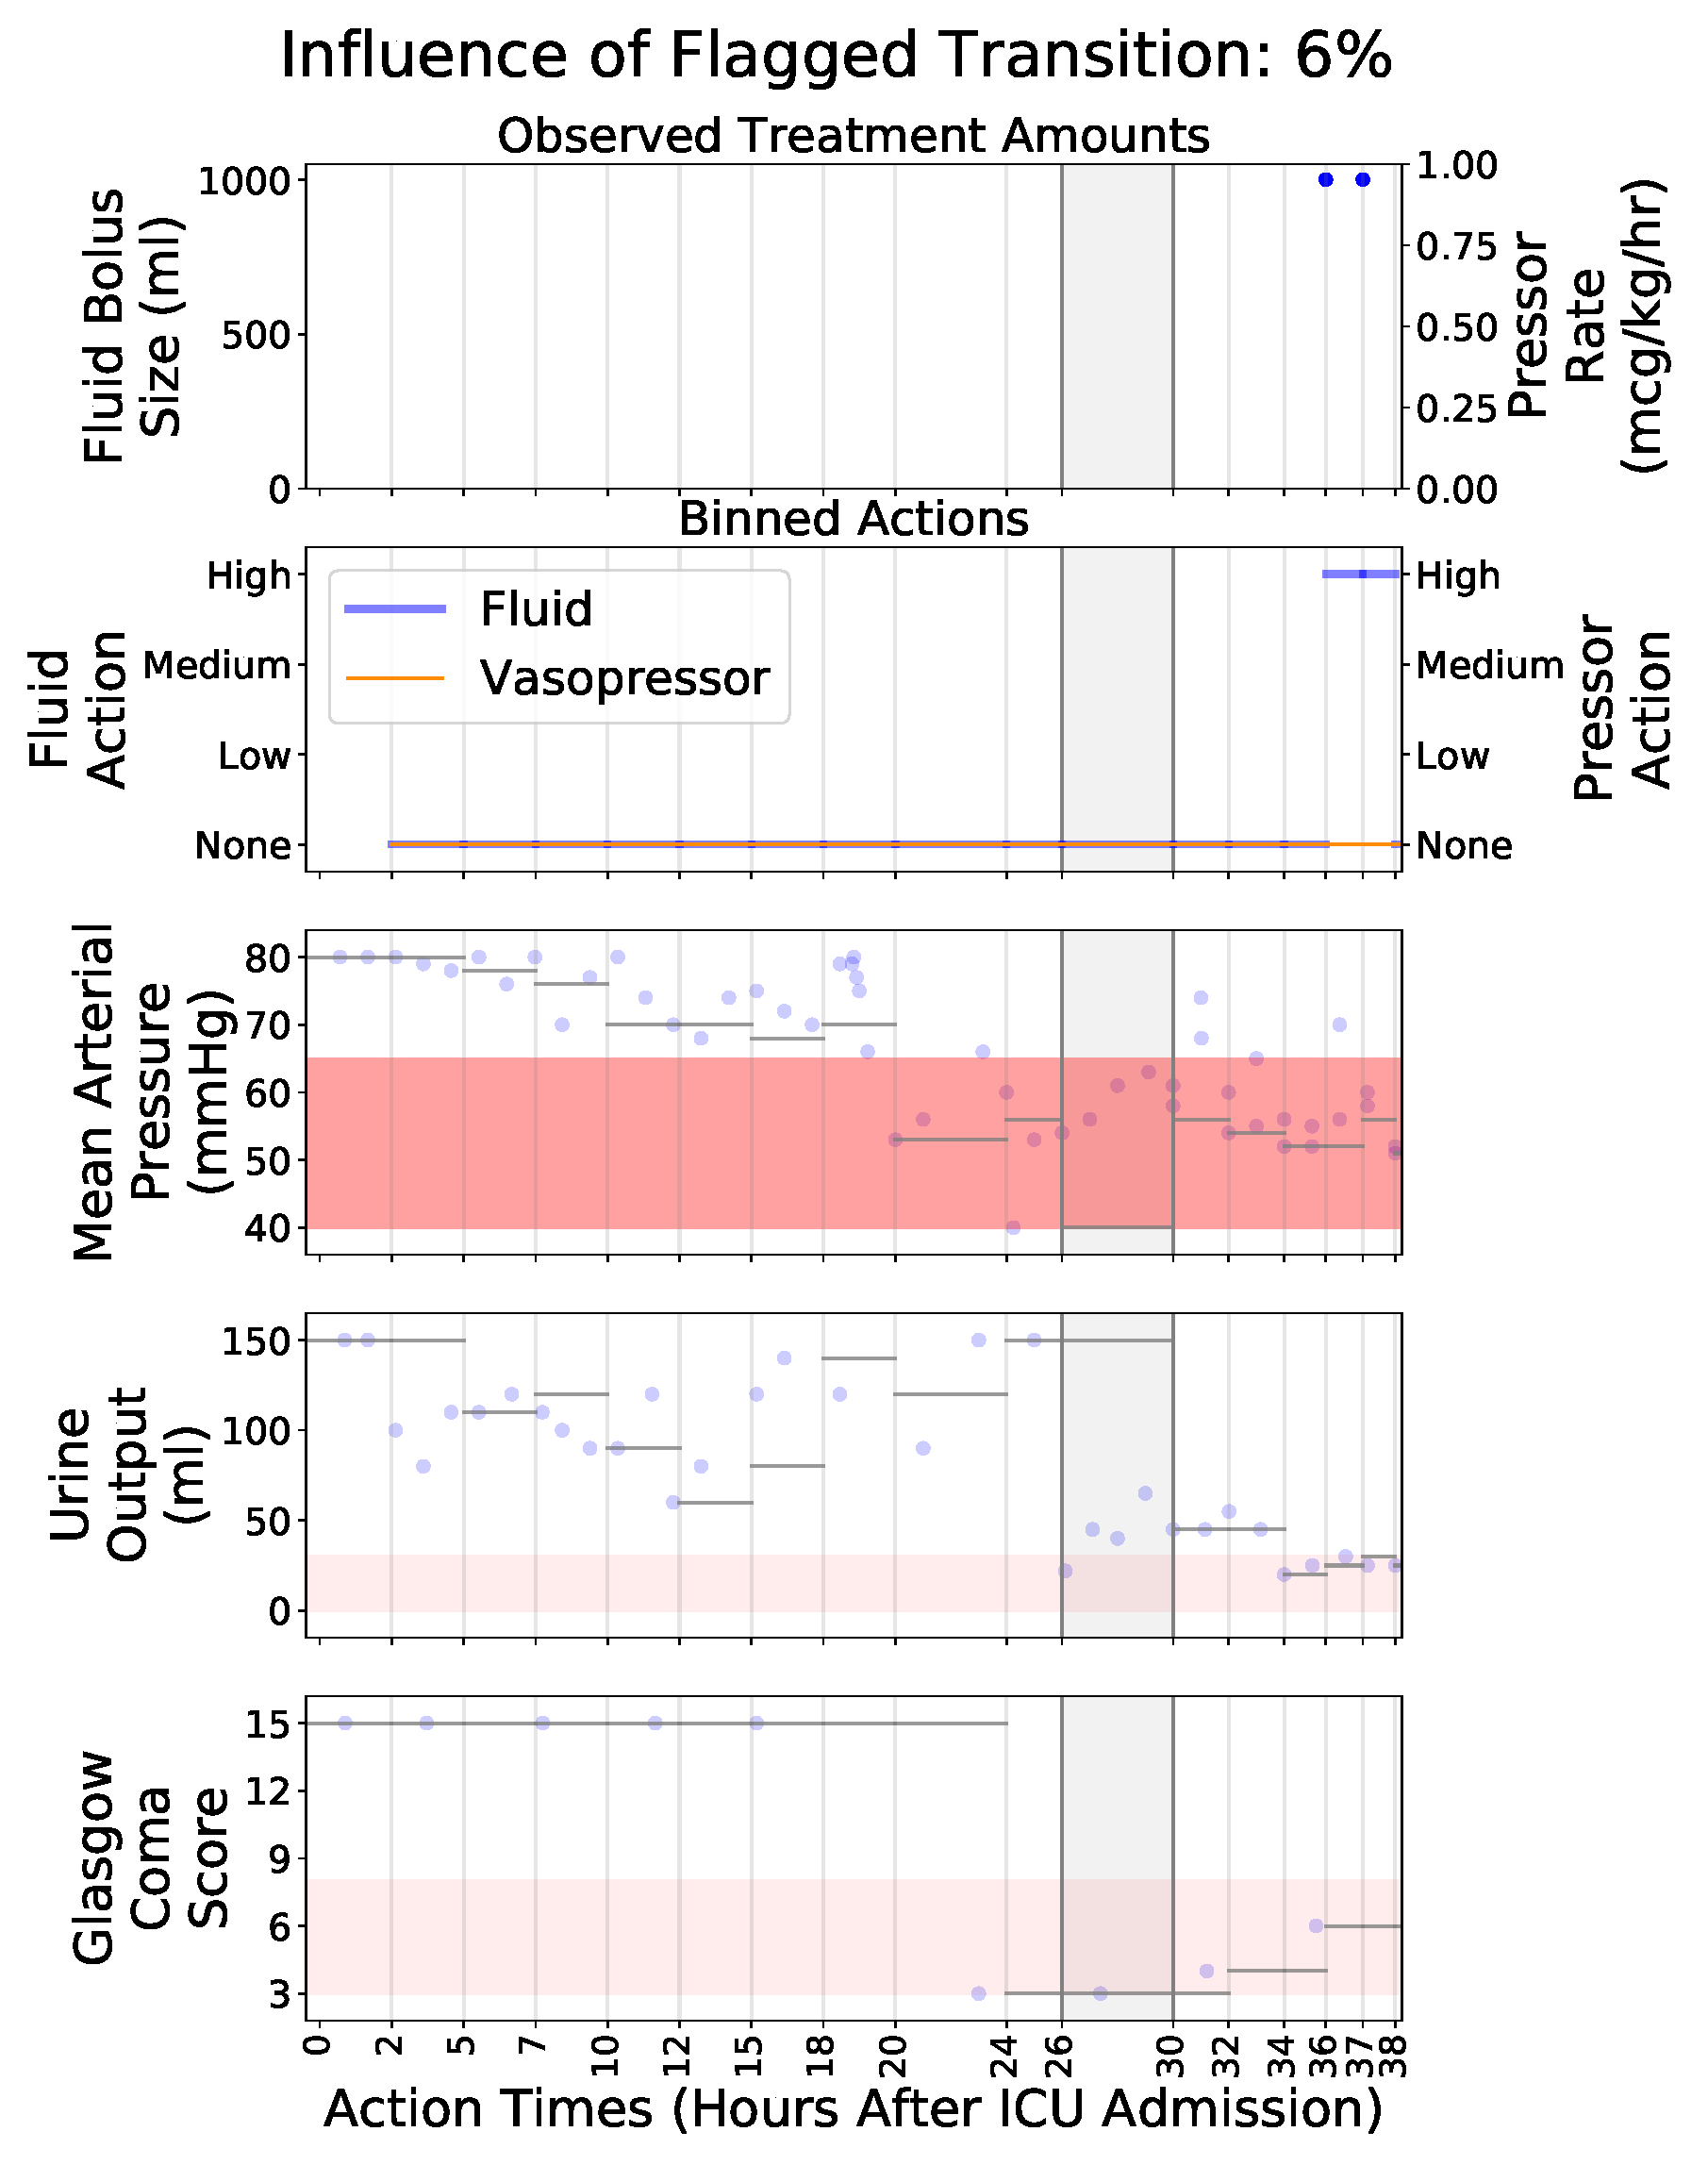
\includegraphics[width=0.45\textwidth]{ID-201525_trans-9.pdf}
\caption{An additional example identified by our influence analysis as having an especially high effect on the OPE value estimate.} 
\label{fig:mimic-9}
\end{figure}

\begin{figure}[H]
\centering
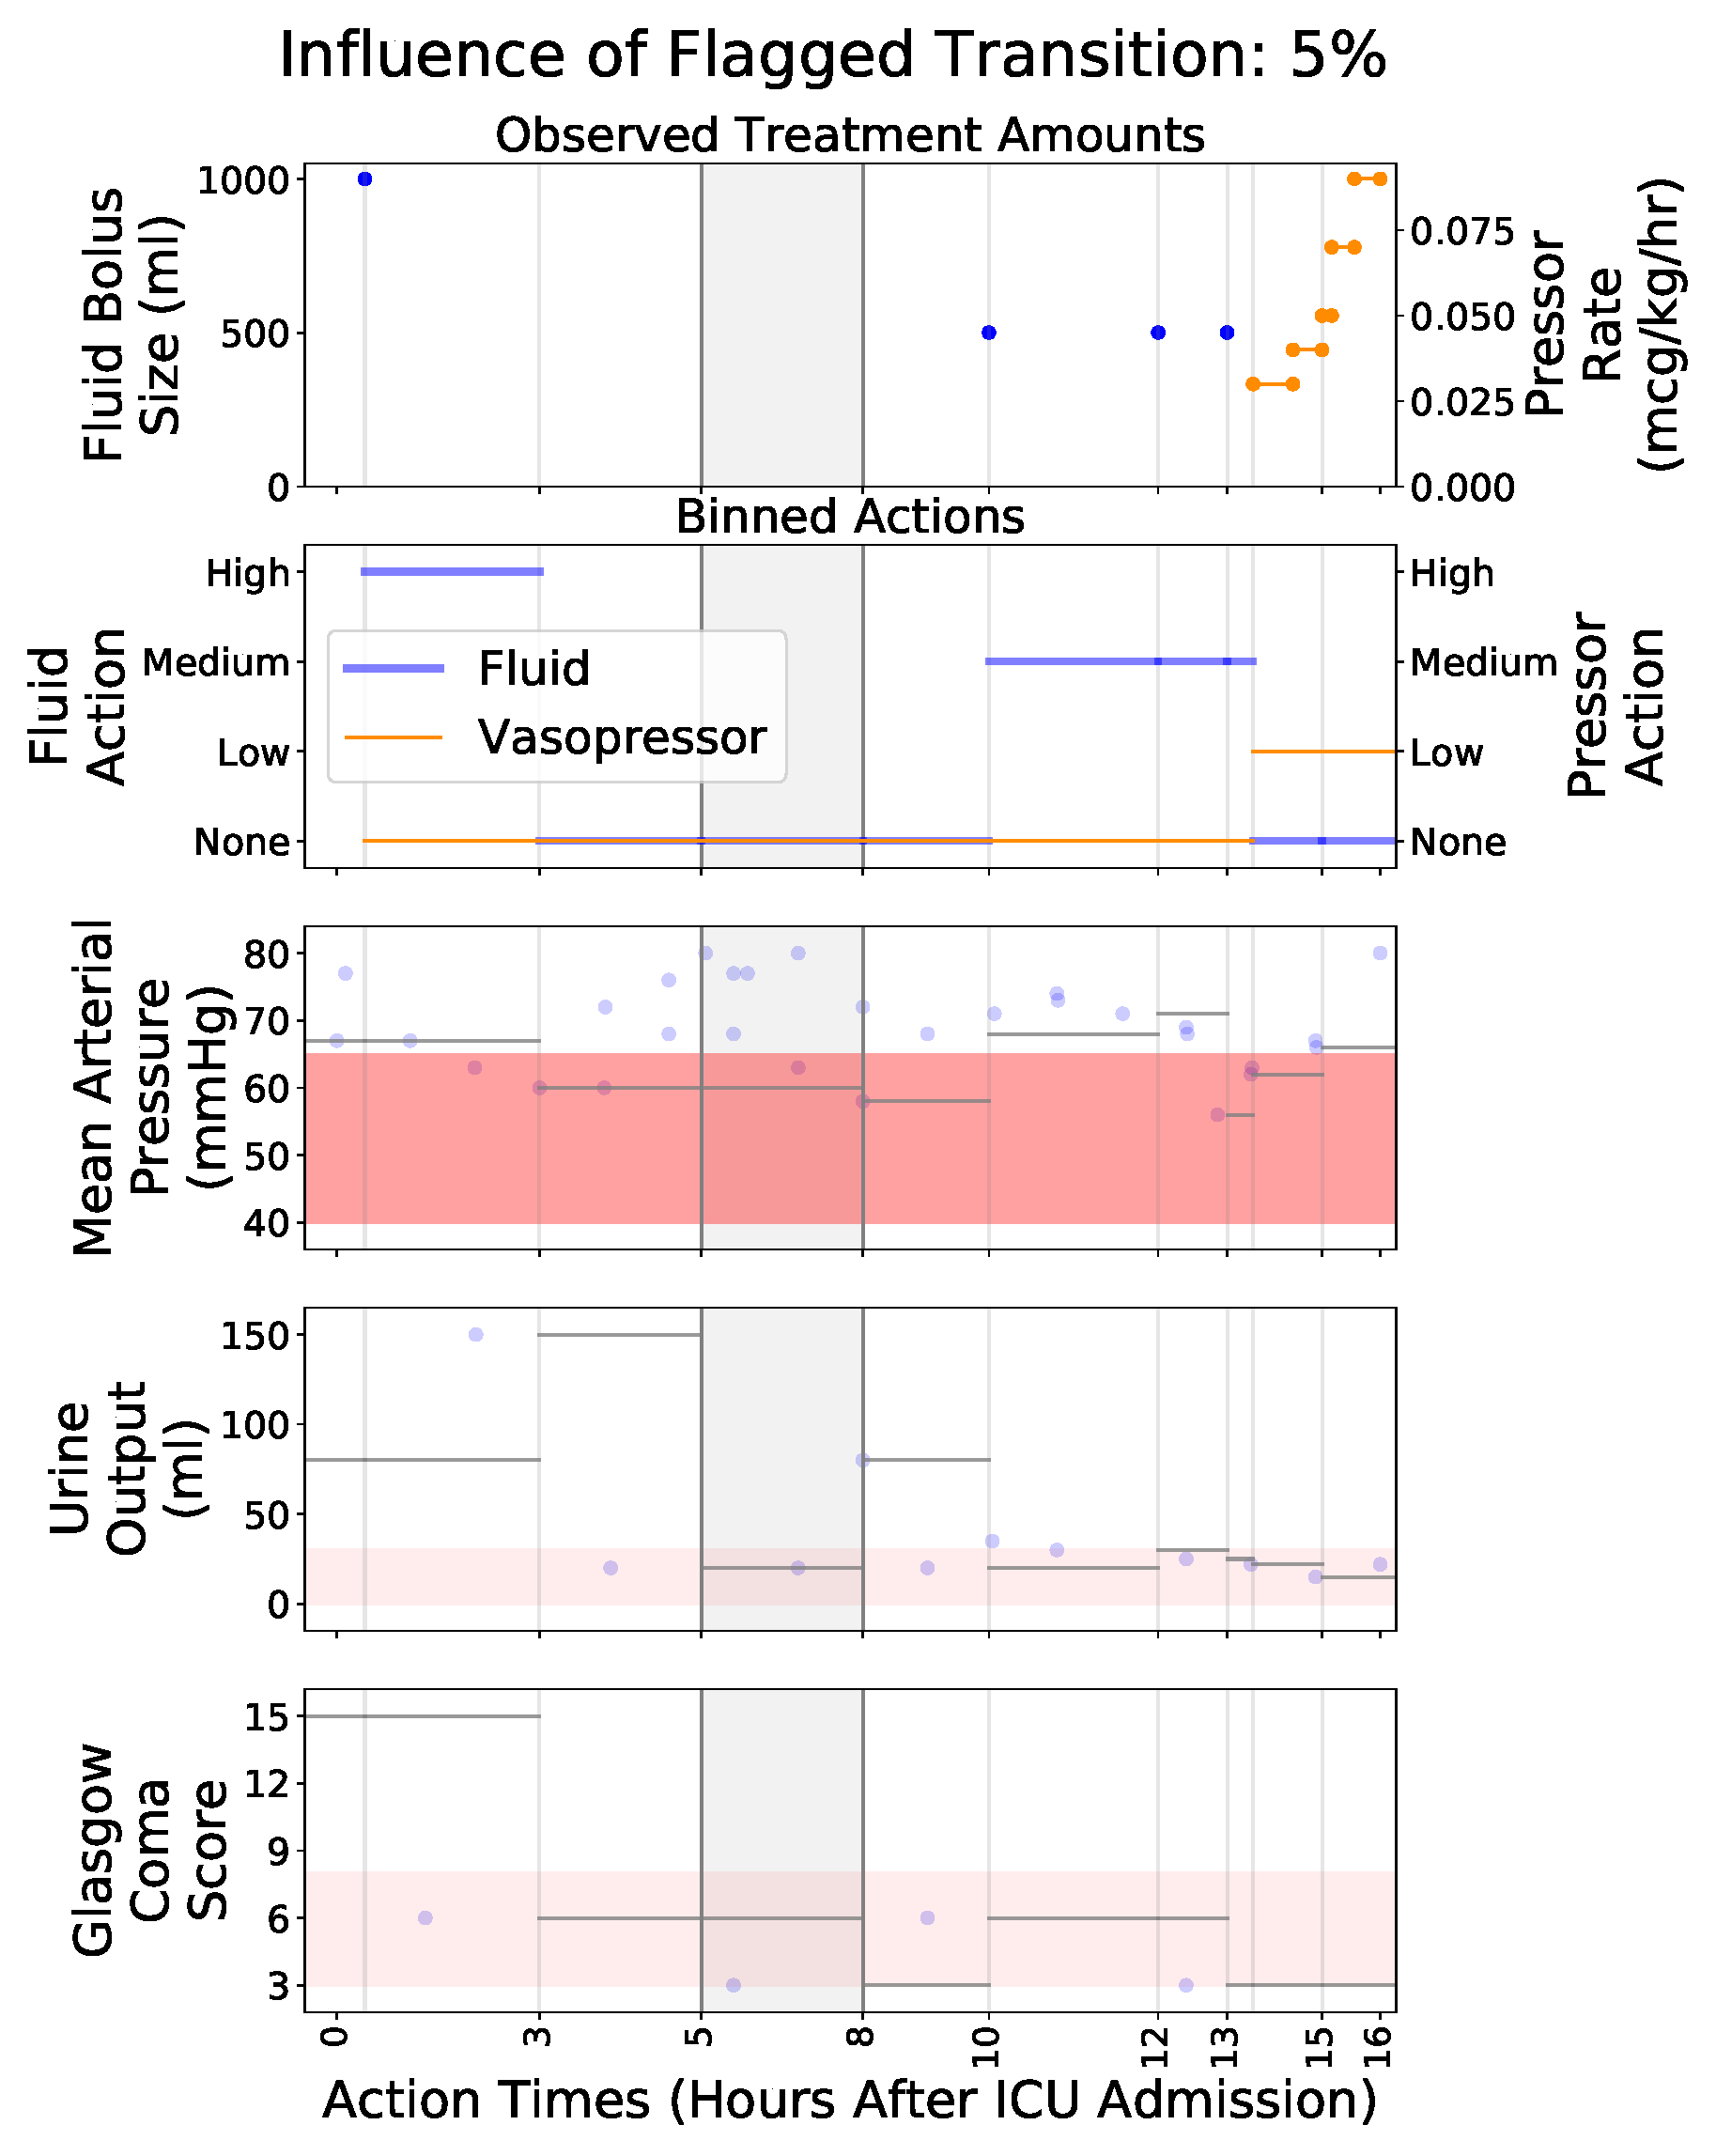
\includegraphics[width=0.45\textwidth]{ID-275864_trans-2.pdf}
\caption{An additional example identified by our influence analysis as having an especially high effect on the OPE value estimate. Note that this transition is from the same trajectory as the influential transition highlighted in Figure \ref{fig:mimic-3}} 
\label{fig:mimic-2}
\end{figure}

\begin{figure}[H]
\centering
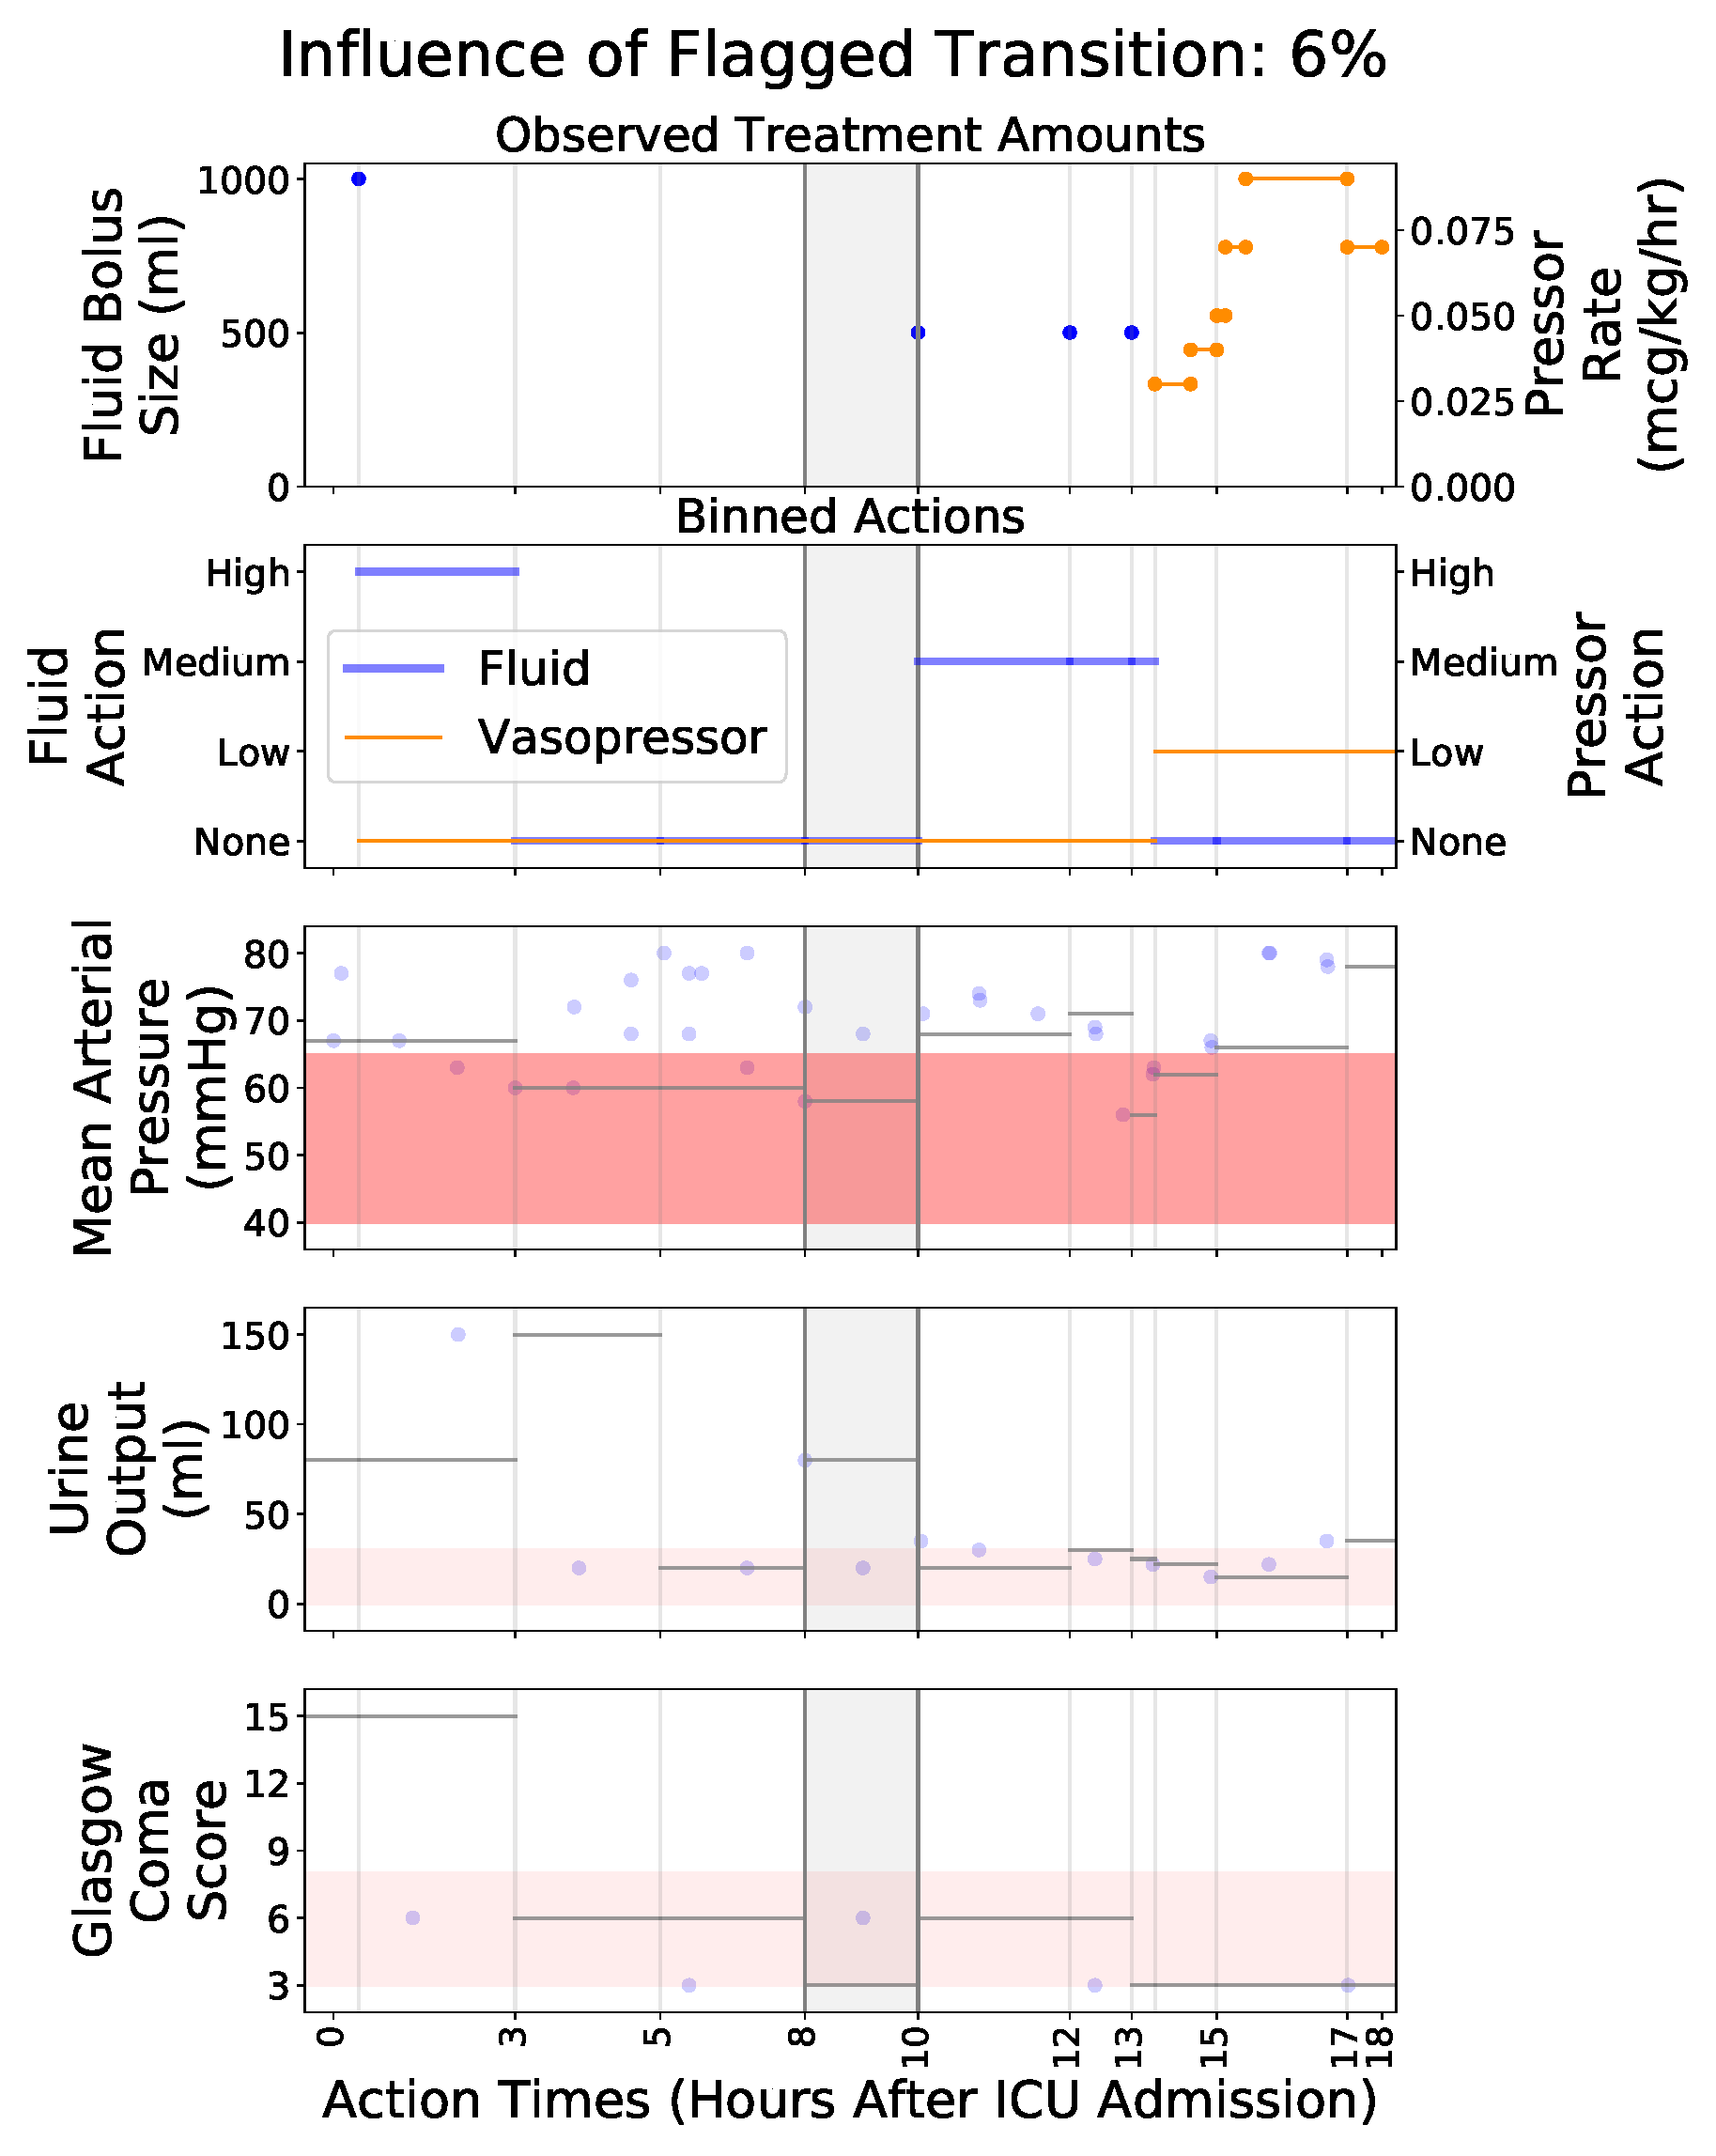
\includegraphics[width=0.45\textwidth]{ID-275864_trans-3.pdf}
\caption{An additional example identified by our influence analysis as having an especially high effect on the OPE value estimate. Note that this transition is from the same trajectory as the influential transition highlighted in Figure \ref{fig:mimic-2}} 
\label{fig:mimic-3}
\end{figure}

\begin{figure}[H]
\centering
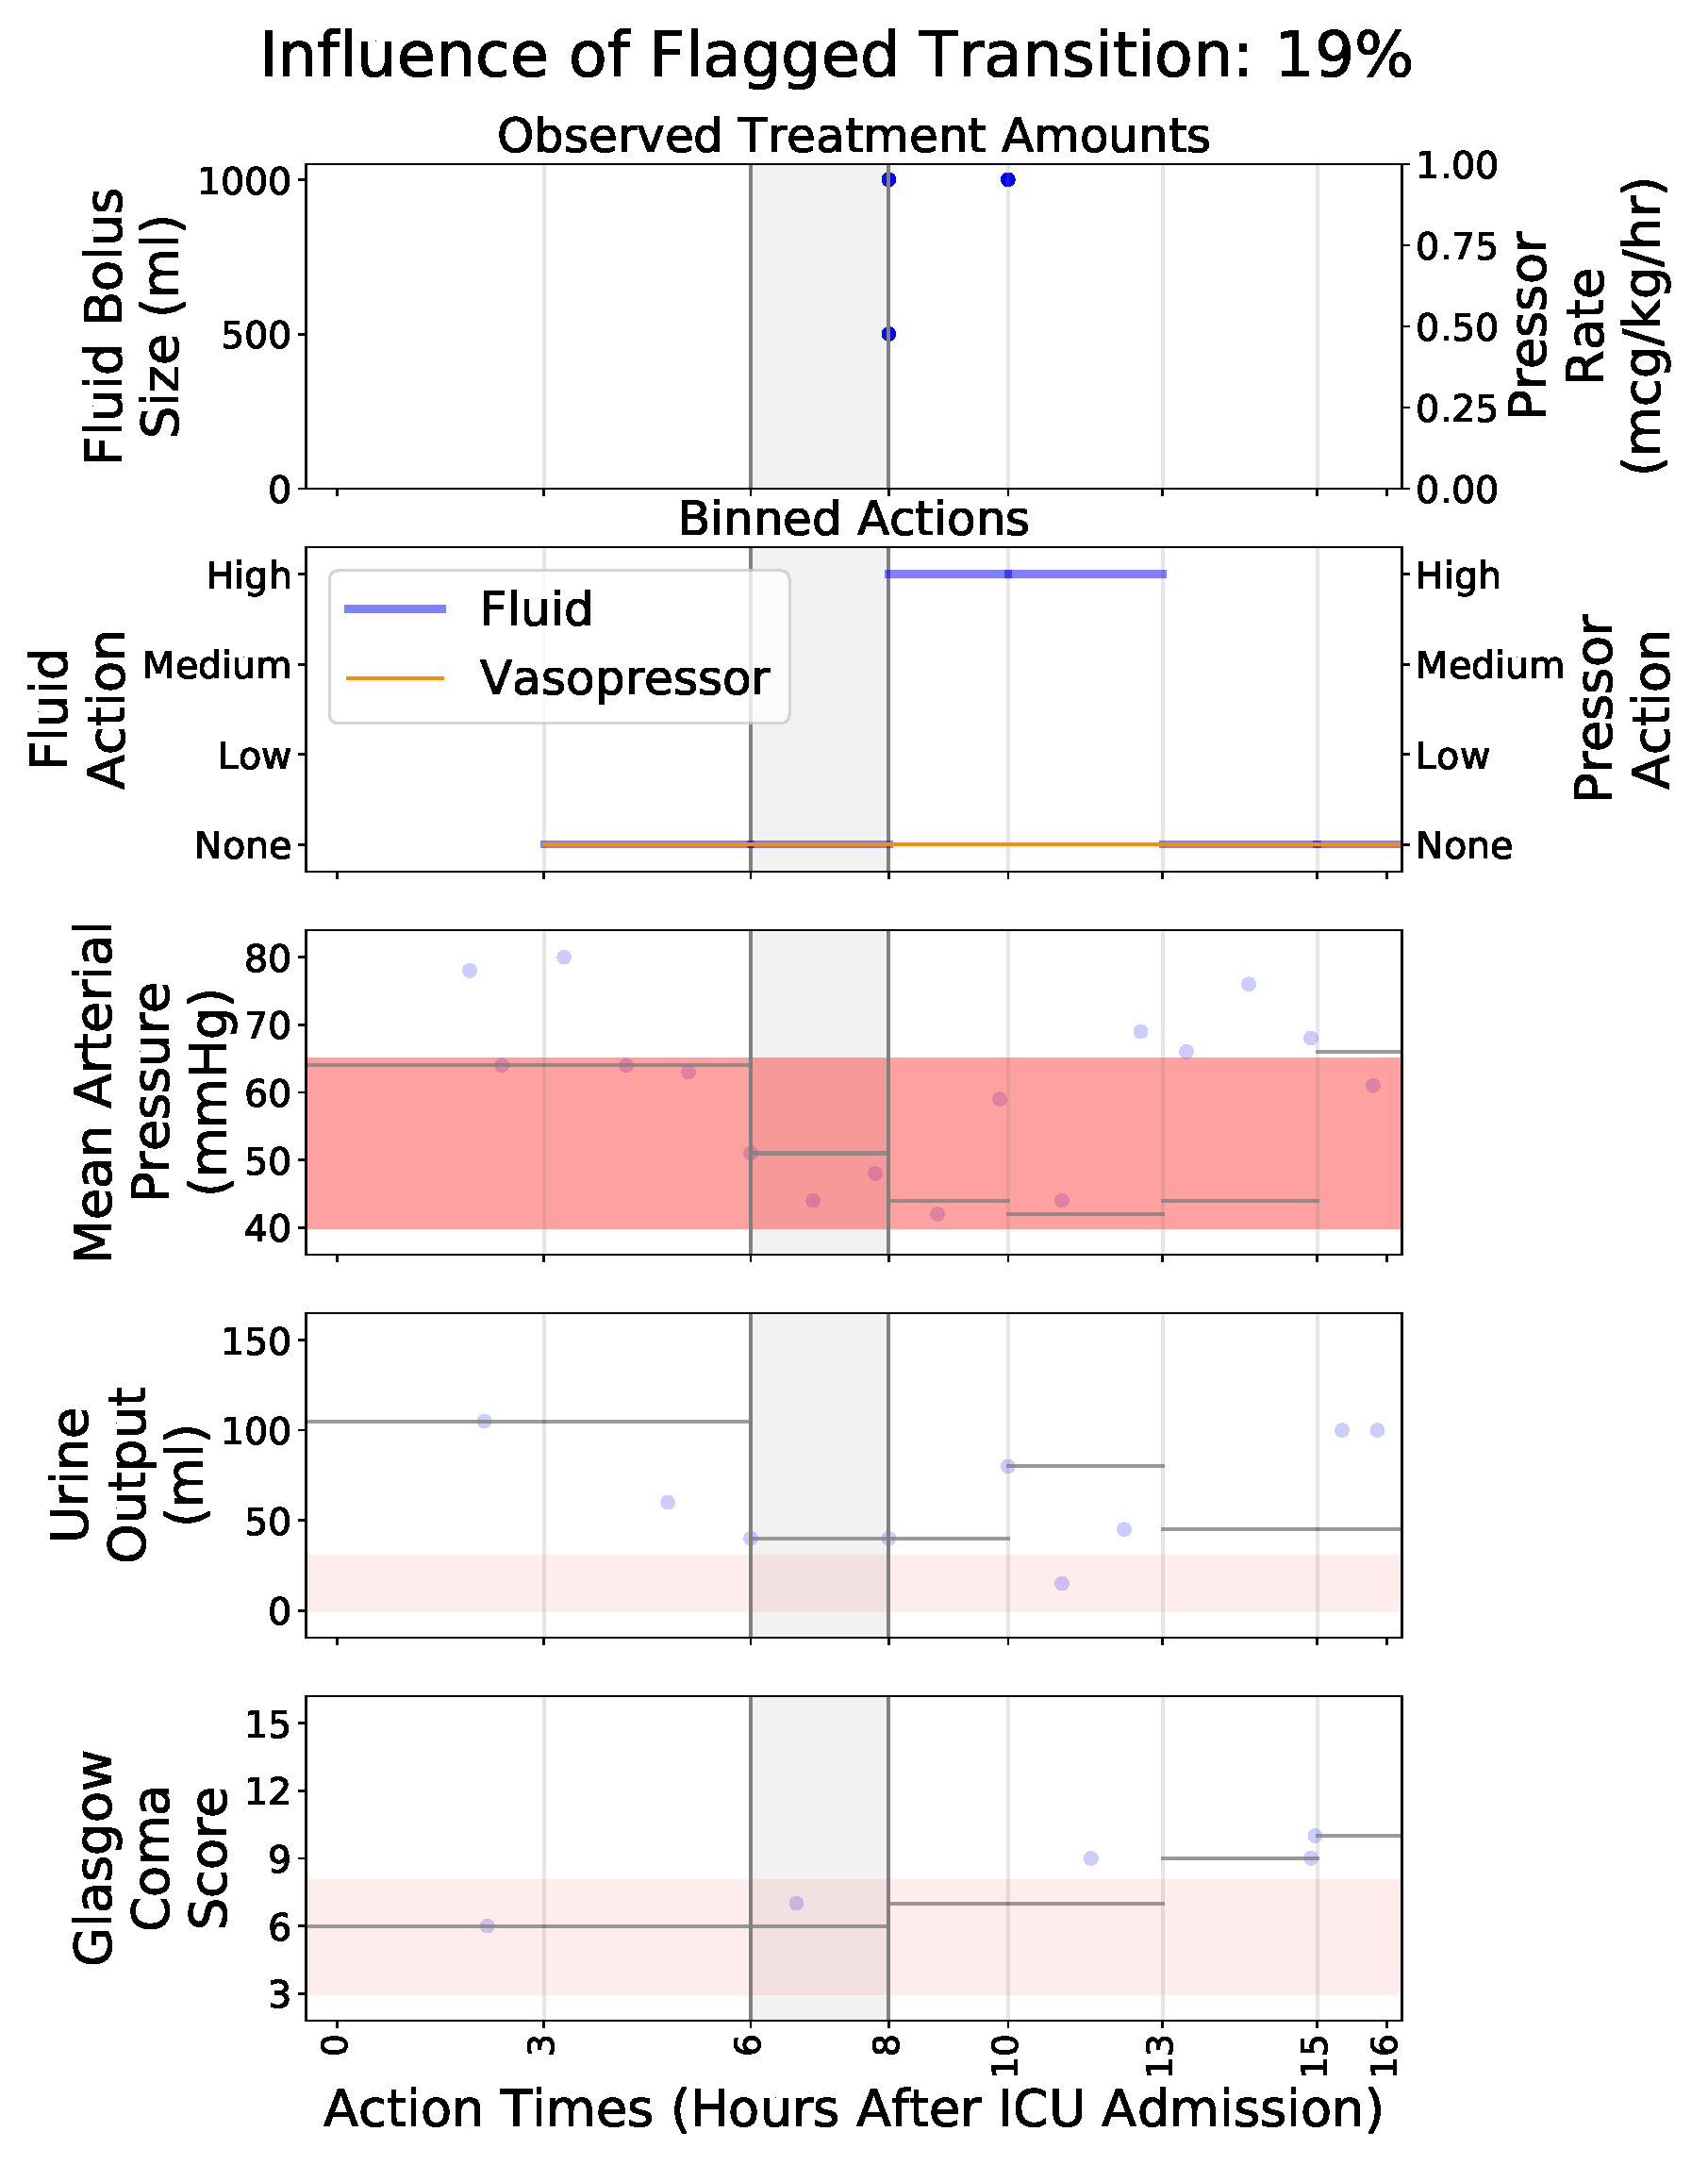
\includegraphics[width=0.45\textwidth]{ID-254228_trans-1.pdf}
\caption{An additional example identified by our influence analysis as having an especially high effect on the OPE value estimate.} 
\label{fig:mimic-1}
\end{figure}

\newpage
\bibliography{references}
\bibliographystyle{icml2020}
\end{document}